\documentclass[3p, authoryear]{elsarticle} %review=doublespace preprint=single 5p=2 column
%%% Begin My package additions %%%%%%%%%%%%%%%%%%%
\usepackage[hyphens]{url}

  \journal{Submitted to Journal} % Sets Journal name


\usepackage{lineno} % add
\providecommand{\tightlist}{%
  \setlength{\itemsep}{0pt}\setlength{\parskip}{0pt}}

\usepackage{graphicx}
%%%%%%%%%%%%%%%% end my additions to header

\usepackage[T1]{fontenc}
\usepackage{lmodern}
\usepackage{amssymb,amsmath}
\usepackage{ifxetex,ifluatex}
\usepackage{fixltx2e} % provides \textsubscript
% use upquote if available, for straight quotes in verbatim environments
\IfFileExists{upquote.sty}{\usepackage{upquote}}{}
\ifnum 0\ifxetex 1\fi\ifluatex 1\fi=0 % if pdftex
  \usepackage[utf8]{inputenc}
\else % if luatex or xelatex
  \usepackage{fontspec}
  \ifxetex
    \usepackage{xltxtra,xunicode}
  \fi
  \defaultfontfeatures{Mapping=tex-text,Scale=MatchLowercase}
  \newcommand{\euro}{€}
\fi
% use microtype if available
\IfFileExists{microtype.sty}{\usepackage{microtype}}{}
\usepackage{natbib}
\bibliographystyle{apalike}
\usepackage{longtable,booktabs,array}
\usepackage{calc} % for calculating minipage widths
% Correct order of tables after \paragraph or \subparagraph
\usepackage{etoolbox}
\makeatletter
\patchcmd\longtable{\par}{\if@noskipsec\mbox{}\fi\par}{}{}
\makeatother
% Allow footnotes in longtable head/foot
\IfFileExists{footnotehyper.sty}{\usepackage{footnotehyper}}{\usepackage{footnote}}
\makesavenoteenv{longtable}
\usepackage{graphicx}
\ifxetex
  \usepackage[setpagesize=false, % page size defined by xetex
              unicode=false, % unicode breaks when used with xetex
              xetex]{hyperref}
\else
  \usepackage[unicode=true]{hyperref}
\fi
\hypersetup{breaklinks=true,
            bookmarks=true,
            pdfauthor={},
            pdftitle={Determining DBSCAN-Entrpopy Hybrid Algorithm Parameters for Converting GPS Points to Activities},
            colorlinks=false,
            urlcolor=blue,
            linkcolor=magenta,
            pdfborder={0 0 0}}
\urlstyle{same}  % don't use monospace font for urls

\setcounter{secnumdepth}{5}
% Pandoc toggle for numbering sections (defaults to be off)

% Pandoc citation processing

% Pandoc header
\usepackage{booktabs}
\usepackage{booktabs}
\usepackage{longtable}
\usepackage{array}
\usepackage{multirow}
\usepackage{wrapfig}
\usepackage{float}
\usepackage{colortbl}
\usepackage{pdflscape}
\usepackage{tabu}
\usepackage{threeparttable}
\usepackage{threeparttablex}
\usepackage[normalem]{ulem}
\usepackage{makecell}
\usepackage{xcolor}



\begin{document}
\begin{frontmatter}

  \title{Determining DBSCAN-Entrpopy Hybrid Algorithm Parameters for Converting GPS Points to Activities}
    \author[Brigham Young University]{Gillian Riches\corref{1}}
   \ead{martingillian4@gmail.com} 
    \author[Brigham Young University]{Gregory Macfarlane\corref{2}}
   \ead{gregmacfarlane@byu.edu} 
      \address[Brigham Young University]{Civil and Environmental Engineering Department, 232 Engineering Building, Provo, Utah 84602}
      \cortext[1]{Corresponding Author}
    \cortext[2]{Present affiliation: Committee Chair}
  
  \begin{abstract}
  
  \end{abstract}
   \begin{keyword} GPS Data, Trips, Clusters\end{keyword}
 \end{frontmatter}

\hypertarget{question}{%
\section{Question}\label{question}}

Global Positioning System (GPS) surveys have become a more accurate and reputable alternative to previous travel survey methods that collect activity-travel patterns. Despite GPS devices' ability to record time and positional characteristics, they still require two steps, cleaning and processing, in order to convert the positional characteristics into trip purposes and activities.

Currently, many researchers use time and speed rule-based algorithms to define when and where activities occur \citep{reviewOfMethods2014}. Due to their subjective nature, these rules are not ideal. For example, people walk at different speeds, so the speed threshold at which someone is considered stagnant would require manual changing from person to person. If not changed, the number of activities for each person could be misleading and inaccurate. These issues may explain why rule-based algorithms' accuracies typically range from 43\% to 61\% \citep{reviewOfMethods2014}. While these processing results (Step 2) are not ideal, the data-cleaning method (Step 1) still serves as a reputable guide regardless of the processing method.

Therefore, once the data is cleaned with accordance to rule-based algorithm methods, a DBSCAN and entropy based algorithm should be applied for the processing step. In this type of algorithm, four parameters are needed to determine an activity: minimum number of points (minpts) within a predefined radius (eps) with a minimum amount of entropy (entr\_t) \citep{GongInspiration}, and after a certain period of time from the previous activity (delta\_t) . When selected properly, these parameters will not need to change from person to person and therefore often lead to more accurate activity counts. In fact, one experiment \citep{DBAlgorithm2017} using just a DBSCAN cluster-based algorithms proved to be 92\% precise.

One way to select the minPoints and radius (eps) thresholds is to arbitrarily pick the minPoints based on how large the data set is (with a minimum of three) and then set k = minPts in a k-distance plot \citep{RKNNMethod2018}. Good values of the radius value is where the k-distance plot shows a strong bend. Another method involves calculating the arithmetic mean and standard deviation of a synthetic GPS trajectory, and subject those values to a Gaussian curve equation to solve for eps given an arbitrary minPts \citep{GaussianMethod2009}. Unfortunately, these methods only work in a pure DBSCAN algorithm where only minpts and eps are accounted for, not entr\_t and delta\_t.

Hence, the purpose of this paper is to explore a method of how to simultaneously select all four parameters as accurately as possible in a DBSCAN entropy based algorithm after the GPS data has been cleaned.

\hypertarget{methods}{%
\section{Methods}\label{methods}}

\hypertarget{data}{%
\subsection{Data}\label{data}}

The GPS data used to determine the four most accurate parameters come from 60 volunteers in
the Utah County area and were taken over a period of six or more months depending on the person. An example of what the raw GPS data looked like is shown in Figure 2.1.

\begin{longtable}[t]{rlrrrr}
\caption{\label{tab:Figure1}Raw GPS Data}\\
\toprule
accuracy & timestamp & speed & lat & lon & time\\
\midrule
16 & 2021-03-17 22:59:36 & -1 & 40.25293 & -111.6602 & 1.616044e+12\\
16 & 2021-03-17 22:59:37 & -1 & 40.25293 & -111.6602 & 1.616044e+12\\
16 & 2021-03-17 22:59:38 & -1 & 40.25293 & -111.6602 & 1.616044e+12\\
16 & 2021-03-17 22:59:39 & -1 & 40.25293 & -111.6602 & 1.616044e+12\\
16 & 2021-03-17 22:59:40 & -1 & 40.25293 & -111.6602 & 1.616044e+12\\
\addlinespace
16 & 2021-03-17 22:59:41 & -1 & 40.25293 & -111.6602 & 1.616044e+12\\
\bottomrule
\end{longtable}

Before the GPS data can be processed, it had to be cleaned and reformatted. Since a DBSCAN algorithm is being used, the speed variable was removed completely. From there, the dates and times had to be reformatted using functions from the \textbf{lubridate} package in R and by writing a ``Yesterday'' function with output ``ActivityDay'' that defines activity days as being from 3 AM to 3 AM instead of 12 AM to 12 AM. This was done because many respondents are college students, so they are likely to make trips after midnight. Table 2.2 shows what the cleaned data looked like.

\begin{longtable}[t]{rrllll}
\caption{\label{tab:Figure2}Cleaned GPS Data}\\
\toprule
lat & lon & timestamp & date & time & activityDay\\
\midrule
40.25293 & -111.6602 & 2021-03-17 22:59:36 & 2021-03-17 & 22:59:36 & 17-3\\
40.25293 & -111.6602 & 2021-03-17 22:59:37 & 2021-03-17 & 22:59:37 & 17-3\\
40.25293 & -111.6602 & 2021-03-17 22:59:38 & 2021-03-17 & 22:59:38 & 17-3\\
40.25293 & -111.6602 & 2021-03-17 22:59:39 & 2021-03-17 & 22:59:39 & 17-3\\
40.25293 & -111.6602 & 2021-03-17 22:59:40 & 2021-03-17 & 22:59:40 & 17-3\\
\addlinespace
40.25293 & -111.6602 & 2021-03-17 22:59:41 & 2021-03-17 & 22:59:41 & 17-3\\
\bottomrule
\end{longtable}

\hypertarget{models}{%
\subsection{Models}\label{models}}

Once the data is cleaned and properly formatted, it is run through a DBSCAN-entropy hybrid algorithm largely based on the method created by Gong et al.~in 2018 \citep{GongInspiration}. After the DBSCAN algorithm determines how many total clusters there are based on the eps and minpts parameters, they get further split based on the delta\_t parameter if necessary. If the time difference between points at the same place is greater than delta\_t, then the points will be split into two separate clusters or activities.

Finally, there is an entropy calculation step where entropy is determined by the change in departure angle between consecutive points. The equation for this entropy is shown in the equation below \citep{GongInspiration}. If the points are in a line, the entropy is very low. In this algorithm, the entr\_t parameter determines at which entropy someone is actually likely to be moving and not just at a stoplight, etc.

\begin{equation}
  EI_q = -\sum_{d=1}^D ((\frac{n_d}{N})ln(\frac{n_d}{N}))
\end{equation}

For this experiment, I will look at a map of the unprocessed, cleaned data and determine with my eyes how many clusters there are. Then, the hybrid algorithm will calculate the number of clusters using randomized values for the four parameters. Based on all the previous research that has been discussed, the ranges for the possible parameters are as follows:

minpts: (3,10)
eps: (1,50)
delta\_t: (300, 1500) seconds
entr\_t: (0.5,3)

Then, I will compare the amount of clusters I saw to the number of clusters the hybrid algorithm calculated. This process was repeated 5 times over 10 different days in order to determine which parameters are the most accurate.

\hypertarget{findings}{%
\section{Findings}\label{findings}}

The hybrid algorithm returned a tibble with the parameters randomly selected for each round. In this case, 5 rounds of parameters were performed for each date. The first 10 rows of the resulting tibble, called random\_clusters when one runs ``tar\_make()'', is shown below:

\begin{verbatim}
## # A tibble: 5 x 7
##      eps minpts delta_t entr_t  draw params    clusters        
##    <dbl>  <int>   <dbl>  <dbl> <int> <list>    <list>          
## 1 11.0        1    8.08   1.25     1 <dbl [4]> <tibble [4 x 4]>
## 2  0.170      1   70.6    2.02     2 <dbl [4]> <tibble [4 x 4]>
## 3  3.10       1  194.     1.79     3 <dbl [4]> <tibble [4 x 4]>
## 4 28.7        1  850.     1.89     4 <dbl [4]> <tibble [4 x 4]>
## 5 31.0        1   80.8    2.10     5 <dbl [4]> <tibble [4 x 4]>
\end{verbatim}

As seen from the random\_clusters object, the number of clusters and information about those clusters are stored as tibbles in the column ``clusters''. An example of the contents of one of those ``clusters'' tibbles is seen in Figure 1.

\begin{verbatim}
## [[1]]
## # A tibble: 4 x 4
##   date       data              n         clusters      
##   <date>     <list>            <list>    <list>        
## 1 2020-09-04 <sf [17,814 x 6]> <int [1]> <sf [148 x 6]>
## 2 2020-09-05 <sf [28,800 x 6]> <int [1]> <sf [254 x 6]>
## 3 2020-09-06 <sf [12,182 x 6]> <int [1]> <sf [31 x 6]> 
## 4 2020-09-08 <sf [16,472 x 6]> <int [1]> <sf [159 x 6]>
\end{verbatim}

Figure 1 also shows the 10 dates that were analyzed for this report as well as the associated nested geometric GPS locations (data) and nested number of clusters (clusters). Further expanding the clusters column list in Figure 1 shows the number of clusters for that date using the parameters from the corresponding iteration. In other words, each date had its number of clusters calculated using 5 different sets of parameters.

Finally, those number of clusters (activities) were all compared to the number of clusters seen by looking at a map of the raw GPS points created using the \emph{leaflet} and \emph{sf} packages in R (example shown in Figure 2). The error between the algorithm's calculated clusters for each set of parameters and the clusters seen from the maps was calculated. Whichever set of parameters consistently gave the lowest error for each date is decidedly the most accurate set of parameters to use for this DBSCAN entropy hybrid algorithm.

\begin{verbatim}
## [[1]]
\end{verbatim}

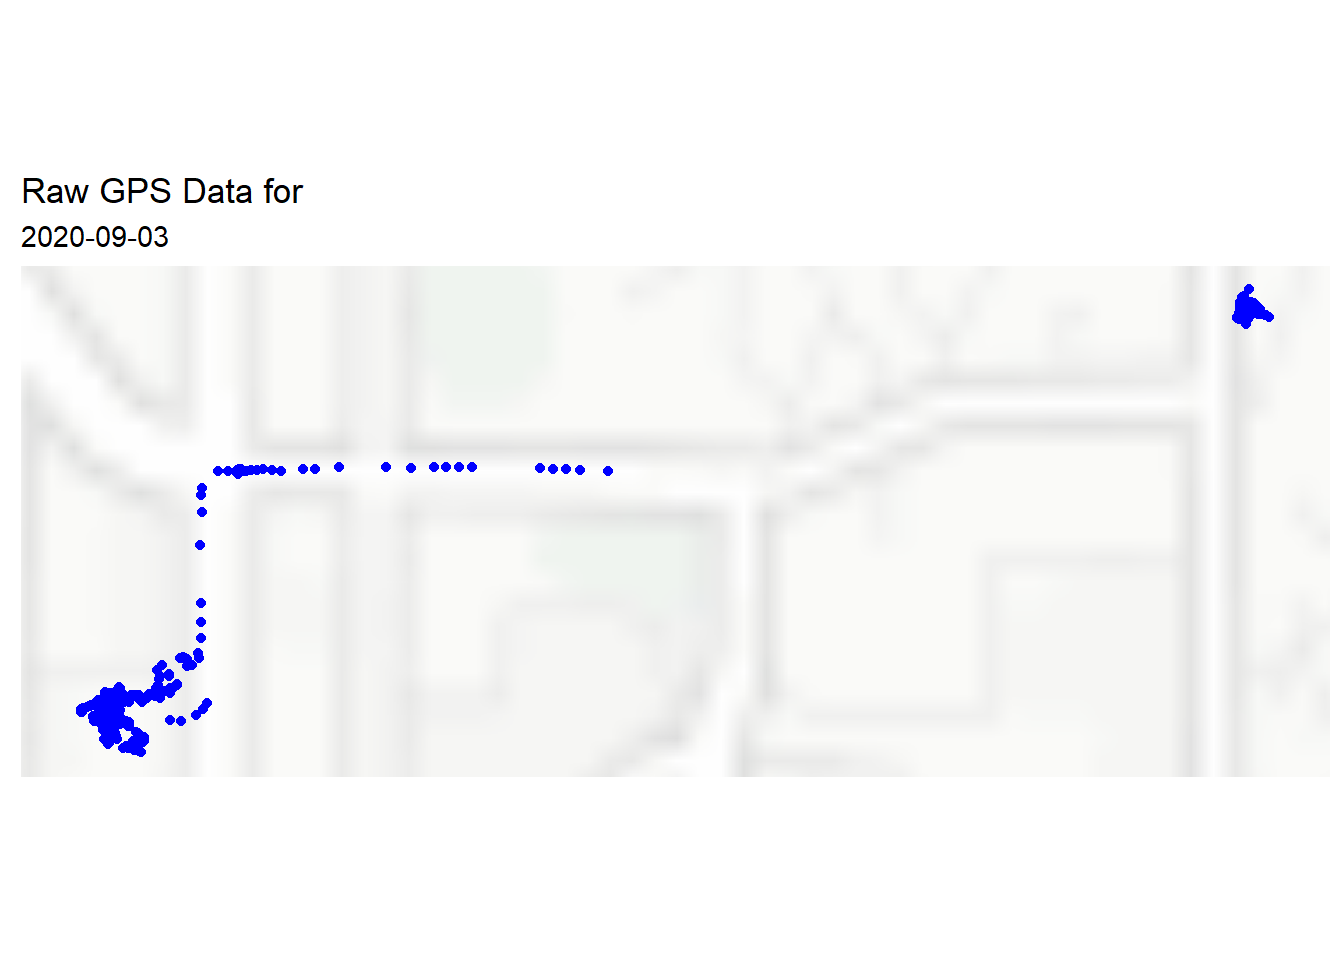
\includegraphics{CellGPSDataToTrips_files/figure-latex/exampleMap-1.pdf}

Based on the results shown in Table 2, the parameters eps = , minpts = , delta\_t, and entr\_t = consistently gave the smallest errors across all 10 days. Therefore, that set of four parameters together are the most accurate to use in this kind of DBSCAN Entropy hybrid method where all four are being used simultaneously, impacting each other, in order to convert cellular GPS data into activities. An important note is that this is based on only performing 5 random iterations of parameters samples. In theory, there are many more combinations of all four of these parameters within their given ranges, so more testing could provide even more accurate results.

\begin{longtable}[t]{rrrrrllll}
\caption{\label{tab:exampleError}Algorithm vs. Manual Error}\\
\toprule
eps & minpts & delta\_t & entr\_t & draw & date & alg\_clusters & man\_clusters & error\\
\midrule
11.00 & 1 & 8.08 & 1.25 & 1 & 9/4/2020 &  &  & \\
0.17 & 1 & 70.60 & 2.02 & 2 & 9/4/2020 &  &  & \\
3.10 & 1 & 194.00 & 1.79 & 3 & 9/4/2020 &  &  & \\
28.70 & 1 & 850.00 & 1.89 & 4 & 9/4/2020 &  &  & \\
31.00 & 1 & 80.80 & 2.10 & 5 & 9/4/2020 &  &  & \\
\addlinespace
11.00 & 1 & 8.08 & 1.25 & 1 & 9/5/2020 &  &  & \\
\bottomrule
\end{longtable}

\hypertarget{acknowledgements}{%
\section*{Acknowledgements}\label{acknowledgements}}
\addcontentsline{toc}{section}{Acknowledgements}

\bibliography{book.bib}


\end{document}
